\documentclass[11pt]{article}
\usepackage[T1]{fontenc}
\usepackage[a4paper,margin=29mm]{geometry}
\usepackage{amsmath,amsthm,mathtools}
\usepackage{newtxtext,newtxmath}
\usepackage{microtype}
\usepackage{enumitem}
\usepackage{tikz}
\usetikzlibrary{arrows.meta,positioning,calc}
\usepackage{xcolor}
\definecolor{linkblue}{RGB}{28,67,112}
\usepackage[colorlinks=true,allcolors=linkblue,bookmarksnumbered=true]{hyperref}
\usepackage[nameinlink,capitalise,noabbrev]{cleveref}
\hypersetup{pdftitle={Arithmetic Stein-degree bounds for log Calabi--Yau pairs},pdfauthor={OpenAI}}
\numberwithin{equation}{section}
\newtheorem{theorem}{Theorem}[section]
\newtheorem{proposition}[theorem]{Proposition}
\newtheorem{lemma}[theorem]{Lemma}
\newtheorem{corollary}[theorem]{Corollary}
\theoremstyle{definition}
\newtheorem{definition}[theorem]{Definition}
\newtheorem{remark}[theorem]{Remark}
\newcommand{\Q}{\mathbb Q}
\newcommand{\Z}{\mathbb Z}
\newcommand{\Pj}{\mathbb P}
\newcommand{\A}{\mathbb A}
\newcommand{\kb}{\overline{k}}
\newcommand{\OO}{\mathcal O}
\newcommand{\Supp}{\operatorname{Supp}}
\newcommand{\Spec}{\operatorname{Spec}}
\newcommand{\Pic}{\operatorname{Pic}}
\newcommand{\Gal}{\operatorname{Gal}}
\newcommand{\sdeg}{\operatorname{sdeg}}
\newcommand{\Diff}{\operatorname{Diff}}
\newcommand{\coeff}{\operatorname{coeff}}
\newcommand{\red}{\mathrm{red}}
\newcommand{\num}{\mathrm{num}}
\newcommand{\bir}{\dashrightarrow}
\newcommand{\simq}{\sim_{\Q}}
\newcommand{\cdeg}[2]{c(#1/#2)}
\setlist[itemize]{leftmargin=*,itemsep=3pt,topsep=5pt}
\setlist[enumerate]{leftmargin=*,itemsep=3pt,topsep=5pt}
\emergencystretch=2em
\title{Arithmetic Stein-degree bounds\\for log Calabi--Yau pairs}
\author{OpenAI}
\date{September 25, 2026}
\begin{document}
\maketitle
\vspace{-1.5em}
\begin{abstract}
Fix $d\geq1$ and $t>0$. Let $(X,B)$ be an ordinary projective log canonical
$\Q$-pair of dimension $d$ over a characteristic-zero field $k$, with $X$
normal and integral, $H^0(X,\OO_X)=k$, $B$ effective, and $K_X+B\simq0$.
We prove that every prime component $S$ of $B$ with coefficient at least $t$
satisfies $[k_S:k]\leq N(d,t)$, where $k_S$ is the relative algebraic closure
of $k$ in $k(S)$. This also bounds the Stein degree of $S$ over $k$, proving
the contraction-to-a-point formulation of Birkar's Stein-degree conjecture
for ordinary $\Q$-pairs.
\end{abstract}

\section{Introduction}

For a proper integral variety $S$ over a field $k$, the Stein degree over
$k$ is
\[
 \sdeg(S/\Spec k)=\dim_k H^0(S,\OO_S).
\]
The field of global functions measures the finite part of the structural
morphism. Its degree can be large even when the dimension of $S$ is fixed.
The question here is whether a boundary component of a log Calabi--Yau pair
has uniformly bounded Stein degree once its coefficient is bounded away
from zero.

Birkar formulates this question for log Calabi--Yau fibrations in
\cite[Conjecture~11.1]{Birkar2026}. Birkar--Qu prove normalized
Stein-degree bounds over algebraically closed characteristic-zero fields
\cite[Theorem~1.3]{BirkarQu2025}, as summarized in
\cite[Theorem~12.1]{Birkar2026}. Over an arbitrary characteristic-zero
field, the finite arithmetic extensions carried by boundary components
must also be controlled.

For any integral $k$-variety $V$, let $k_V$ be the relative algebraic closure
of $k$ in its function field and put
\begin{equation}\label{eq:constants}
 \cdeg{V}{k}=[k_V:k].
\end{equation}
Our result bounds this stronger invariant.

\begin{theorem}\label{thm:main}
For every integer $d\geq 1$ and real number $t>0$, there is an integer
$N(d,t)\geq1$ with the following property. Let $k$ be any field of
characteristic zero, and let $(X,B)$ be a projective log canonical
$\Q$-pair such that
\[
 \dim X=d,\qquad H^0(X,\OO_X)=k,\qquad K_X+B\simq0.
\]
Assume that $X$ is normal and integral and that $B$ is effective. If $S$ is
a prime component of $B$ with coefficient at least $t$, then
\[
 \cdeg{S}{k}\leq N(d,t).
\]
Consequently
\[
 \sdeg(S/\Spec k)\leq
 \dim_k H^0(S^\nu,\OO_{S^\nu})
 =\cdeg{S}{k}\leq N(d,t),
\]
where $S^\nu$ is the normalization of $S$.
\end{theorem}

\Cref{thm:main} thus proves the contraction-to-$\Spec k$ formulation of
Birkar's Stein-degree conjecture for ordinary $\Q$-pairs.

The birational strategy follows Birkar--Qu \cite{BirkarQu2025}, using the
minimal model program (MMP), bounded complements, and boundedness of
Fano varieties. Two additional arguments address the arithmetic and
inductive difficulties. First, \cref{sec:arithmetic} turns geometric
boundedness into a bound on Galois orbits of divisorial valuations. A bounded
extension fixes a polarization class; a determinant construction descends
a bounded power of that class. On a resolution of the resulting bounded
pair, a log canonical place is determined by a stratum and integral
weights. The finite permutation action on strata therefore bounds its
arithmetic orbit, even though there may be infinitely many such places.
Second, when the distinguished divisor becomes vertical on a Mori fibre
space, the earlier bigness of that divisor forces a horizontal boundary
component of coefficient one. A relative MMP makes the two components
intersect, so ordinary divisorial adjunction reduces the dimension
(\cref{sec:preparation,sec:proof}).

\section{Conventions and foundational inputs}

All fields have characteristic zero. A variety is integral and of finite
type over its ground field. A contraction is a projective surjective
morphism $f:V\to Z$ between normal varieties with $f_*\OO_V=\OO_Z$.
Divisors over a variety are identified with divisorial valuations,
normalized to have value group $\Z$. We use log discrepancies:
\[
 a(P,X,B)=1-\coeff_P B_W,
 \qquad K_W+B_W=p^*(K_X+B).
\]
The pair is log canonical (lc) if these numbers are nonnegative and
Kawamata log terminal (klt) if they are positive. A divisorial valuation
of log discrepancy zero is an \emph{lc place}. A variety is
$\epsilon$-lc if the pair with zero boundary has all log discrepancies
at least $\epsilon$. Canonical divisors in birational comparisons are
chosen compatibly. The relation $\simq0$ means that a positive integral
multiple is a principal Cartier divisor.

We require $\Q$-factoriality only over the working field. It need not hold
over an algebraic closure. For normal geometrically integral varieties,
the singularity conditions just stated are preserved by ground-field
extension: resolve in characteristic zero, base change, and apply the
log smooth discrepancy criterion. Coefficients on geometric components
are unchanged.

\subsection{Constants and generic fibres}

\begin{lemma}\label{lem:constants}
Let $V$ be an integral $k$-variety.
\begin{enumerate}[label=\textup{(\roman*)}]
\item The number $\cdeg{V}{k}$ is the number of irreducible components of
$V_{\kb}$; these components form one Galois orbit. It is a birational
invariant. If $V$ is proper, then $H^0(V,\OO_V)\subseteq k_V$, with
equality when $V$ is normal.
\item If $V\to Z$ is dominant and $Z$ is geometrically integral over $k$,
then, for its generic fibre,
\begin{equation}\label{eq:generic-constants}
 \cdeg{V}{k}\leq\cdeg{V_{\eta_Z}}{k(Z)}.
\end{equation}
\item If $X$ is normal projective and $H^0(X,\OO_X)=k$, then $X$ is
geometrically integral. The normal base of a contraction from $X$ is
also geometrically integral. Its generic fibre is normal, projective,
and has global functions $k(Z)$.
\end{enumerate}
\end{lemma}

\begin{proof}
The extension $k_V/k$ is finite and separable, and $k(V)/k_V$ is regular.
Its embeddings in $\kb$ give precisely the geometric components. Properness
makes global functions finite over $k$. On a normal variety every element
of $k(V)$ algebraic over $k$ is integral over every local ring and hence
regular, proving (i).

The regular extension $k(Z)/k$ is linearly disjoint from $k_V/k$. Thus
$k_Vk(Z)$ is a degree-$[k_V:k]$ extension of $k(Z)$ inside $k(V)$ and is
contained in the relative algebraic closure of $k(Z)$ there. This proves
(ii). The first assertion of (iii) follows from (i). For a contraction,
global functions on the base are $k$ and localizing $f_*\OO_X=\OO_Z$
gives the asserted generic-fibre function field. Normality is preserved
by localization, and a normal variety over a perfect field is geometrically
normal; the assertion follows over $k(Z)$ as well.
\end{proof}
We use $\cdeg{P}{k}$ for a divisorial valuation by using its residue
function field. Its geometric extensions on a model where it is a divisor
are distinct valuations forming a single Galois orbit.

If $(X,B)$ is as in \cref{thm:main} and $X\to Z$ is a contraction,
restriction to the generic fibre gives a projective lc log Calabi--Yau
pair over $k(Z)$. Indeed, work over the smooth locus of $Z$, restrict a
log resolution, and use generic smoothness and adjunction. The same
argument restricts a specified principal multiple of $K_X+B$. Hence a
horizontal boundary component can be treated by induction in the
dimension of this generic fibre, using \eqref{eq:generic-constants}.

\subsection{Established theorems used in the proof}

We state the versions needed, so that no arithmetic strengthening of a
geometric boundedness theorem is implicit.

\begin{itemize}
\item \emph{Klt MMP and extraction.} For a projective morphism of normal
varieties over a characteristic-zero field and a $\Q$-factorial klt pair
$(V,\Delta)$ with effective rational boundary, an MMP with suitable ample
scaling terminates in a Mori fibre space if $K_V+\Delta$ is not relatively
pseudo-effective. If $\Delta$ is relatively big and $K_V+\Delta$ is
relatively pseudo-effective, it terminates in a minimal model. Outputs
are $\Q$-factorial and klt. A finite set of exceptional valuations of
log discrepancy at most one for a klt $\Q$-pair can be extracted by a
projective birational morphism with $\Q$-factorial source and no other
exceptional prime divisors. These are consequences of
\cite{BCHM2010}; versions over the fields used here are
\cite[Theorem~21.7, Corollaries~21.9--21.10, Theorem~22.1]{LyuMurayama}.
We also use the negativity lemma, monotonicity of discrepancies along
a klt MMP, and klt base point freeness.

\item \emph{Bounded complements.} In fixed dimension, for an lc pair over
an algebraically closed characteristic-zero field, with coefficients in
a fixed finite rational set, underlying variety of Fano type, and nef
anti-log canonical divisor, there is an enlarged lc boundary $B^+\geq B$
such that $n(K+B^+)\sim0$, where $n$ depends only on the dimension and
coefficient set. This is the relevant case of
\cite[Theorem~1.7]{Birkar2019}; a finite rational set is contained in an
appropriate hyperstandard set. We may replace $n$ by a prescribed fixed
multiple.

\item \emph{BAB.} For fixed $q$ and $\epsilon>0$, geometrically
$\epsilon$-lc projective Fano varieties of dimension $q$ over an
algebraically closed characteristic-zero field form a bounded family
\cite[Theorem~1.1]{Birkar2021}. In particular, they admit very ample
line bundles of bounded degree.
\end{itemize}

Here Fano type over $Z$ means the existence of an effective rational
boundary $\Delta$ with $(V,\Delta)$ klt and $-(K_V+\Delta)$ ample over
$Z$. The absolute term means $Z=\Spec k$. The other standard inputs are
resolution and principalization in characteristic zero, klt vanishing
and rational singularities, and divisorial adjunction; see
\cite{BMT2011,KM1998,Kollar2013}. We give the index and field arguments
for adjunction in \cref{lem:adjunction}.

The algebraically closed bounds above are uniform in the ground field.
One may also deduce this from their complex versions: descend all finite
data, including resolutions and positivity witnesses, to a finitely
generated field over $\Q$, embed it into $\mathbb C$, and spread and
specialize an embedding or a complement. For an embedding, very ampleness
and its degree persist after shrinking the parameter space. For the
complement used below, the general-member argument in
\cref{lem:complement} gives the same transfer in its specified linear
system.

\begin{lemma}\label{lem:crepant}
Suppose $(V,D)$ is lc and $K_V+D\simq0$. Under a birational contraction
or flip, push $D$ forward and keep compatible canonical divisors. Then
the resulting pair is crepant to $(V,D)$, remains lc with effective
boundary, and retains every specified relation $n(K_V+D)\sim0$.
\end{lemma}

\begin{proof}
Write the specified multiple as the divisor of a rational function.
Since the map extracts no divisors, pushing forward gives the same
principal-divisor identity on the new model. Its two pullbacks to a
common resolution are that same principal divisor. Thus the pullbacks
agree, which proves crepancy and the discrepancy assertions. Without a
specified multiple, choose one first.
\end{proof}

\section{Arithmetic consequences of geometric boundedness}\label{sec:arithmetic}

\subsection{Descending a complement}

\begin{lemma}\label{lem:complement}
Fix $d$ and a rational number $b\in(0,1)$. There is an integer $n=n(d,b)$
such that the following holds over every characteristic-zero field $k$.
Suppose $V$ is a normal geometrically integral projective klt Fano
variety of dimension $d$, $S$ is a $\Q$-Cartier prime divisor,
$(V,bS)$ is lc, and $-K_V-bS$ is nef. Then there is an effective rational
boundary $C\geq bS$ over $k$ with
\[
 (V,C)\text{ lc},\qquad n(K_V+C)\sim0.
\]
We may assume $nb\in\Z$.
\end{lemma}

\begin{proof}
Apply bounded complements to $(V_{\kb},bS_{\kb})$ and multiply the index
by the denominator of $b$. The geometric complement has the form
$bS_{\kb}+D/n$, where
\begin{equation}\label{eq:weil-system}
 D\in|-nK_V-nbS|_{\kb}.
\end{equation}
This linear system is defined over $k$. For clarity, its underlying
space is the space of rational sections of the integral Weil divisor
$-nK_V-nbS$; it can be computed on the smooth locus and extended across
codimension two. Sections commute with field extension. The divisor
is $\Q$-Cartier, although it need not be Cartier.

A general geometric member of \eqref{eq:weil-system} gives an lc pair.
To see this, resolve both $(V,bS)$ and the rational map of this linear
system. On a further resolution the pullbacks of its members have the
form $F+M$, with $F$ fixed and rational and $M$ varying in a base point
free Cartier system. Indeed, differences of pullbacks are divisors of
ratios of sections, so eliminating the base ideal gives precisely this
decomposition. Arrange that the support of $F$ and the crepant boundary
$B_W$ of $(V,bS)$ has simple normal crossings. The existence of one lc
member implies that every coefficient of $B_W+F/n$ is at most one:
adding the effective moving part could not remove an excessive
coefficient. By Bertini, a general $M$ is smooth and transverse to this
support, and its coefficient $1/n$ is at most one. The resulting log
smooth pair is lc.

The argument describes a nonempty geometric open subset of the
projective space of sections. Since $k$ is infinite, its $k$-rational
points are Zariski dense even after extension to $\kb$. Choose a member
$D$ over $k$ in this open subset and set $C=bS+D/n$. Then
$n(K_V+C)=nK_V+nbS+D$ is principal over $k$, as required.
\end{proof}

\subsection{Log canonical places of a simple normal crossings pair}

A stratum of a reduced simple normal crossings divisor will mean an
irreducible component of a nonempty intersection of its components,
including a single component.

\begin{lemma}\label{lem:weights}
Let $W$ be smooth over an algebraically closed field, and let $H$ be a
reduced simple normal crossings divisor. If a divisorial valuation $v$
satisfies $a(v,W,H)=0$, then its centre is a stratum. Moreover, $v$ is
uniquely determined by that stratum and its positive integral values on
the components of $H$ containing the stratum.
\end{lemma}

\begin{proof}
Let $T$ be the centre. If fewer than $\operatorname{codim}T$ components
of $H$ pass through its generic point, complete their local equations
by a smooth hypersurface containing $T$, keeping simple normal
crossings. The enlarged reduced divisor is lc, and the additional
hypersurface has positive value under $v$. The discrepancy for $H$
would therefore be positive. Thus the components through the generic
point of $T$ have number $\operatorname{codim}T$, and $T$ is a stratum.

We prove uniqueness by a sequence of blowups that is determined by the
weights. If $T$ is already a divisor, the normalized valuation centred
at its generic point is its order of vanishing. Otherwise choose two
components through $T$, with values $p_1,p_2>0$, and blow up their
codimension-two intersection near the generic point of $T$. The new
reduced total divisor is simple normal crossings and the blowup is log
crepant. The exceptional divisor has value $\min(p_1,p_2)$; the values
of the two strict transforms are
\[
 p_1-\min(p_1,p_2),\qquad p_2-\min(p_1,p_2),
\]
with a zero value indicating that the centre is not on that strict
transform. The other values are unchanged.

The new centre is again a stratum. These data specify it uniquely over
the generic point of $T$: in the exceptional $\Pj^1$-bundle, the two
strict transforms give the two distinguished sections. Unequal weights
choose one section; equal weights choose the full fibre, since a
different proper subvariety would not be a stratum. Intersecting with
the remaining components through $T$ imposes the remaining prescribed
conditions. This is also immediate in the two blowup charts.
The sum of the positive weights decreases by $\min(p_1,p_2)$. Repeating
therefore reaches a divisorial centre, where the valuation is unique.
Tracing back proves the assertion.
\end{proof}

\begin{corollary}\label{cor:finite-low}
A klt rational pair has only finitely many divisorial valuations of log
discrepancy less than one.
\end{corollary}

\begin{proof}
First work over an algebraic closure and take a log resolution with
crepant boundary $B_W$. Let $H=\sum H_i$ be a reduced simple normal
crossings divisor containing its support, and write $B_W=\sum b_iH_i$,
allowing zero and negative coefficients. Since the pair is klt,
$b_i<1$. For a valuation $v$ with discrepancy less than one,
\begin{equation}\label{eq:weight-discrepancy}
 a(v,W,B_W)=a(v,W,H)+\sum_i(1-b_i)v(H_i)<1.
\end{equation}
The first term on the right is a nonnegative integer, so it is zero.
The centre is therefore a stratum by \cref{lem:weights}. At each
stratum, the positive integral weights satisfy
$\sum_i(1-b_i)v(H_i)<1$, which allows only finitely many choices.
There are finitely many strata, and \cref{lem:weights} gives uniqueness.
Over the original field, each divisorial valuation extends to a
geometric one with the same discrepancy, so finiteness follows there
as well.
\end{proof}

\subsection{Bounded resolutions and Galois orbits}

We record the bounded-family fact needed to keep resolutions over the
field of the data.

\begin{lemma}\label{lem:embedded}
Fix bounds for the ambient projective dimension, the degree of a normal
geometrically integral projective variety $V$, and the degree of a
reduced divisor $D\subset V$, where $D$ may be empty. There are constants
$R,M$ depending only on these bounds such that, over the field of the
embedded pair, one can find a projective resolution $p:W\to V$ and a
geometrically simple normal crossings reduced divisor $H$ containing
the exceptional locus and the strict transform of $D$, with
\[
 b_2(W_{\bar k})\leq R,
 \qquad
 \#\{\text{geometric components and strata of }H\}\leq M.
\]
One may use an $\ell$-adic second Betti number for any $\ell$.
\end{lemma}

\begin{proof}
We explain both the finite-type parametrization and the field assertion.
A reduced pure-dimensional projective locus of dimension $j$ and
degree at most $D_0$ in a fixed $\Pj^N$ is cut out set-theoretically by
equations of bounded degree. Indeed, given a geometric point outside
the locus, choose a linear projection to $\Pj^{j+1}$ whose centre
misses the locus and whose fibre through that point misses it. Such a
choice exists by the usual dimension count. The projection is finite
on the locus; its image is a hypersurface of degree at most $D_0$.
Pulling back its equation separates the point. Multiplying by forms
nonvanishing at that point puts these equations in one fixed degree.
The codimension-one case uses the identity projection; the empty and
full loci require no argument. A basis of the space of equations in
this fixed degree has bounded size. These spaces of equations descend
to the field of the locus, because extension of the ground field
commutes with their defining linear conditions.

Apply this to $V$ and $D$. Tuples of equations of bounded size and
degree give parameter spaces of finite type over $\Q$ containing all
the embedded pairs over their original fields. Stratify to take
fibrewise reductions and to impose geometric normality, integrality,
dimension, and the divisor condition. This can be done by spreading
the reductions at generic points and shrinking, using characteristic
zero and generic flatness, and then proceeding by Noetherian induction.

At the generic point of each stratum, resolve the pair over that
point's own function field. Resolution and principalization in
characteristic zero may be chosen to give geometric simple normal
crossings, with no extension of that function field
\cite[Theorems~1.3 and~6.1, including the Addendum]{BMT2011}. Spread the projective morphism, the reduced divisor,
and a dense open on which the morphism is an isomorphism. After
shrinking, the resolving variety is smooth and projective over the
stratum, the morphism is fibrewise birational, and the divisor has
geometric simple normal crossings in every fibre and contains the
required exceptional and marked loci. To verify the last condition,
spread the inverse image of the closed bad locus and the smoothness
and expected codimensions of intersections of the divisor components;
the components can be considered after an auxiliary finite étale
cover of the parameter stratum for this verification. The resolution
itself remains defined on the original stratum. Noetherian induction
on its complement yields finitely many families.

Every embedded pair over a field is a point of one of these strata,
so pulling back the corresponding family gives a resolution over that
same field. Smooth proper base change bounds the second Betti numbers.
Applying it also to intersections of components, after the finite
étale covers just used, bounds the numbers of their geometric connected
components and hence the numbers of strata. Taking maxima over the
finitely many families gives $R$ and $M$.
\end{proof}

\begin{proposition}\label{prop:bab-orbits}
Fix an integer $q\geq1$, a real $\epsilon>0$, and an integer $n\geq1$.
There is a finite number $A(q,\epsilon,n)$ with the following property.
Let $Q/k$ be a normal geometrically integral projective
$\epsilon$-lc Fano variety of dimension $q$, and suppose
\[
 (Q,\Lambda)\text{ is lc},\qquad \Lambda\geq0,
 \qquad n(K_Q+\Lambda)\sim0.
\]
Then every divisorial valuation $v$ with $a(v,Q,\Lambda)<1$ satisfies
\[
 \cdeg{v}{k}\leq A(q,\epsilon,n).
\]
\end{proposition}

\begin{proof}
\emph{A bounded polarization after a bounded extension.}
By BAB, $Q_{\kb}$ has a very ample line bundle $L$ of bounded degree.
Its space of sections also has bounded dimension: for a nondegenerate
$q$-dimensional projective variety, degree is at least codimension
plus one, so $h^0(L)\leq L^q+q$.

We claim that $\Pic(Q_{\kb})$ is free abelian of bounded rank. First a
numerically trivial line bundle $N$ on $Q_{\kb}$ is trivial. Indeed,
klt singularities are rational, so Euler characteristics can be computed
on a resolution; Riemann--Roch there gives
$\chi(N)=\chi(\OO_{Q_{\kb}})$. Klt Kawamata--Viehweg vanishing applies
to both bundles, since $N-K_Q$ and $-K_Q$ are ample. Hence
$h^0(N)=h^0(\OO_{Q_{\kb}})=1$. The divisor of a nonzero section of $N$
is effective and numerically trivial. Its intersection with a power
of an ample divisor forces it to be zero, so $N$ is trivial.

Pullback to a resolution therefore embeds $\Pic(Q_{\kb})$ into the
Néron--Severi group modulo numerical equivalence of that resolution:
numerical triviality of a pullback implies numerical triviality
downstairs by lifting curves and the projection formula. This is a
free abelian group of rank at most the second Betti number.
\Cref{lem:embedded}, applied to the bounded embedding with empty
marking, bounds that number. This proves the claim.

The Galois action on this lattice has finite image, because its finitely
many generators are defined over finite extensions. Finite subgroups
of $\operatorname{GL}_r(\Z)$ have bounded order for bounded $r$:
reduction modulo $3$ is injective on each such subgroup. To recall why,
the kernel has no nontrivial finite-order element. If
$I+3^aM$ with $a\geq1$ and $M\not\equiv0\pmod3$ had prime order,
the binomial expansion at that prime would have a nonzero lowest
$3$-adic term; every finite-order element has a power of prime order.
Thus an extension $F/k$ of bounded degree fixes the class of $L$.

Invariance of a class need not descend a line bundle, so one more step
is necessary. Put $r=h^0(L)$. Choose a finite Galois field of definition
of $L$ over $F$, and isomorphisms between its conjugates. Their failure
to satisfy the cocycle condition consists of scalar factors. On
\begin{equation}\label{eq:determinant-descent}
 L^{\otimes r}\otimes\bigl(\det H^0(L)\bigr)^{-1}
\end{equation}
these factors cancel: a scalar acts to the $r$th power on both factors.
This gives effective descent data. The required isomorphisms exist
over the chosen field of definition because two line bundles that
become isomorphic over an algebraic closure are already isomorphic
over that field on a proper geometrically integral variety: apply
base change to the sections of their quotient and its inverse.
Consequently \eqref{eq:determinant-descent} descends to a line bundle
$A$ on $Q_F$ whose geometric class is $L^{\otimes r}$. It is very ample
and has bounded degree and bounded $h^0(A)$.

\emph{A bounded marked support.}
The principal-divisor identity implies that $n\Lambda$ is integral,
since $K_Q$ is an integral Weil divisor. Thus every positive coefficient
of $\Lambda$ is at least $1/n$. On the geometric variety,
\begin{equation}\label{eq:marked-degree}
 (\Supp\Lambda)_{\red}\cdot A^{q-1}
 \leq n(-K_Q)\cdot A^{q-1}
 \leq n\bigl((q-1)A^q+2\bigr).
\end{equation}
For the last inequality, intersect $q-1$ general members of $|A|$.
When $q>1$ they give a smooth curve avoiding the singular locus of
the normal variety, and adjunction says
\[
 (-K_Q)\cdot A^{q-1}=(q-1)A^q+2-2g\leq(q-1)A^q+2.
\]
For $q=1$ the same formula is the usual degree formula on a smooth
curve. Hence the embedded pair $(Q_F,(\Supp\Lambda)_\red)$ satisfies
the hypotheses of \cref{lem:embedded} with uniform bounds.

\emph{The orbit of a valuation.}
Choose the resolution supplied there over $F$, and write
$K_W+B_W=p^*(K_Q+\Lambda)$. Its geometric reduced divisor $H$ contains
the support of $B_W$. Since $(Q,\Lambda)$ is lc, $B_W\leq H$.
For every geometric extension $\bar v$ of $v$,
\[
 0\leq a(\bar v,W_{\kb},H)
 \leq a(\bar v,W_{\kb},B_W)<1.
\]
The left-hand discrepancy is integral, hence zero. By
\cref{lem:weights}, $\bar v$ is determined by its centre stratum and
its weights on the components of $H$. The Galois subgroup over $F$
that fixes all the geometric components and strata fixes each such
valuation: its centre and weights cannot change. There are at most
$M$ objects in this finite set, so each orbit over $F$ has size at most
$M!$. Its full orbit over $k$ has size at most $[F:k]M!$. These are
uniformly bounded, proving the proposition.
\end{proof}


\section{Birational preparation and adjunction}\label{sec:preparation}

\subsection{Making the distinguished component positive}

\begin{lemma}\label{lem:klt-model}
For $(X,B)$ as in \cref{thm:main}, there is a projective birational
morphism $h:Y\to X$ with $Y$ $\Q$-factorial and klt such that the
crepant boundary $B_Y$ is effective. The strict transform of every
component of $B$ has its original coefficient.
\end{lemma}

\begin{proof}
Take a projective resolution and run a relative $K$-MMP with ample
scaling over $X$. In this birational setting every divisor class,
including the zero boundary, is big over $X$: the generic fibre is a
point. The big-boundary MMP applies. A Mori fibre space over $X$
cannot be an output, since its total space is birational to $X$,
whereas its base would have smaller dimension and still dominate $X$.
We therefore obtain a $\Q$-factorial klt minimal model $h:Y\to X$.
Write
\[
 K_Y+B_Y=h^*(K_X+B).
\]
Minimality says that $-B_Y$ is nef over $X$, and $h_*B_Y=B\geq0$.
The negativity lemma gives $B_Y\geq0$. Crepancy proves the remaining
assertions.
\end{proof}

\begin{lemma}\label{lem:positive-component}
Let $X$ be a $\Q$-factorial klt projective variety, $(X,B)$ an effective
lc pair with $K_X+B\simq0$, and $S$ a component of coefficient at
least $t>0$. Fix a rational $b$ with $0<b<t$. There is a sequence of
birational MMP steps preserving $S$, followed by a Mori fibre
contraction $X_1\to Z_1$, such that $S_1$ is ample over $Z_1$ and
$(X_1,B_1)$ is an effective lc log Calabi--Yau pair. If $Z_1$ is a
point and $H^0(X,\OO_X)=k$, then
\[
 Z_1=\Spec k,\qquad -K_{X_1}\text{ ample},\qquad
 -K_{X_1}-bS_1\text{ nef}.
\]
\end{lemma}

\begin{proof}
Set $D=K_X+B-bS\simq-bS$. It is not pseudo-effective, since its
intersection with a fixed ample divisor to the power $d-1$ is
negative. Choose an ample rational divisor $H$ and $\delta>0$
rational and small enough that $D+\delta H$ remains outside the
pseudo-effective cone.

There is an effective klt boundary $\Delta$ with
$K_X+\Delta\simq D+\delta H$. Indeed, $(X,B-bS)$ is lc and $X$ is
klt, so $(X,(1-\eta)(B-bS))$ is klt for $0<\eta\ll1$. The class
$\delta H+\eta(B-bS)$ is ample for sufficiently small $\eta$.
Represent it by a general effective rational divisor with small
coefficients, preserving klt, and add this divisor to
$(1-\eta)(B-bS)$.

Run the MMP for $K_X+\Delta$ with scaling by a sufficiently large
multiple $mH$. At a ray $R$ used by the program, including the final
Mori fibre ray, write $L_i=D_i+\delta H_i$ for the transformed class.
The scaling condition gives
\[
 L_i\cdot R<0,\qquad (L_i+\lambda_i mH_i)\cdot R=0,
 \qquad \lambda_i\geq0.
\]
It follows that $\lambda_i>0$, $H_i\cdot R>0$, and hence
$D_i\cdot R<0$. Thus every step is positive on $S_i$. The divisor
$S_i$ cannot be contracted by a divisorial step: if it were, it would
be an effective exceptional divisor nef over that contraction, in
contradiction with the negativity lemma. Flips do not contract divisors.

The resulting Mori fibre contraction has relative Picard number one,
so positivity on its extremal ray makes $S_1$ relatively ample.
\Cref{lem:crepant} gives the assertions about $(X_1,B_1)$. If the base
is a point, the function-field condition makes it $\Spec k$. Now
$\rho(X_1/k)=1$. The nonzero effective divisor $B_1\simq-K_{X_1}$
is ample, and the effective divisor
$B_1-bS_1\simq-K_{X_1}-bS_1$ is nef, as asserted.
\end{proof}

\subsection{Making a vertical prime a pullback}

\begin{lemma}\label{lem:vertical}
Let $U\to Z$ be a contraction with $U$ projective and $\Q$-factorial
of Fano type over $Z$. Let $P$ be a vertical prime divisor. There is a
sequence of $(-P)$-negative MMP steps over $Z$ such that the final
transform $P'$ survives on a $\Q$-factorial klt variety $U'$ and
$-P'$ is semiample over $Z$. If $f:U'\to Z'$ is its
semiample contraction, then $Z'\to Z$ is birational and for some
integer $m>0$ and a nonzero effective Cartier divisor $T$ on $Z'$,
\begin{equation}\label{eq:pullback}
 mP'=f^*T.
\end{equation}
The MMP is an isomorphism over the generic point of $Z$. Every
horizontal prime $E$ therefore survives and meets $P'$; its
normalization has a nonzero effective restricted divisor
$P'|_{E^\nu}$.
\end{lemma}

\begin{proof}
First $-P$ is pseudo-effective over $Z$. Choose an effective Cartier
divisor on $Z$ containing the proper closed image of $P$. A sufficiently
large multiple of its pullback has coefficient at least one along
$P$, so subtracting $P$ leaves an effective divisor.

Choose an effective klt boundary $\Delta$ for which
$L=-(K_U+\Delta)$ is ample over $Z$. For a sufficiently small rational
$a>0$, the class $L-aP$ is also relatively ample. After twisting a
sufficiently divisible multiple by a divisor from $Z$, choose a
general member and divide by that multiple to obtain an effective
rational divisor $D_a\simq L-aP$ over $Z$ with $(U,\Delta+D_a)$ klt.
Then $\Psi=\Delta+D_a$ is big over $Z$, and
\[
 K_U+\Psi\simq-aP\quad\text{over }Z.
\]
The big-boundary MMP with ample scaling terminates in a minimal model
$U'$, since this class is relatively pseudo-effective. Its steps are
$(-P)$-negative. As in \cref{lem:positive-component}, the negativity
lemma prevents the contraction of $P$. The steps are isomorphisms over
a nonempty open subset of $Z$: there $P$ is absent and its negative
has zero intersection with every curve in a fibre. In particular,
every horizontal prime survives.

Put $L'=K_{U'}+\Psi'$, which is nef over $Z$. The boundary $\Psi'$ is
still big over $Z$, so write $\Psi'\simq A'+D'$ over $Z$ with $A'$
relatively ample and $D'\geq0$. For sufficiently small rational
$\eta>0$, the effective boundary
\[
 \Theta'=(1-\eta)\Psi'+\eta D'
\]
is klt and satisfies
\[
 L'-(K_{U'}+\Theta')\simq\eta A'\quad\text{over }Z.
\]
Klt base point freeness applies to a sufficiently divisible nef
Cartier multiple of $L'$ \cite[Theorem~11.1]{LyuMurayama}. Thus $L'$, and consequently $-P'$, is
semiample over $Z$. The relative theorem can also be applied
geometrically and descended: relative generation of sections is
detected by faithfully flat base change.

Let $f:U'\to Z'$ be the associated contraction. On the generic fibre
over $Z$, the line bundle of a multiple of $P'$ is trivial and the
field of global functions is $k(Z)$. Hence $Z'\to Z$ is birational.
Choose $m>0$ such that $mP'$ is Cartier and
$\OO_{U'}(-mP')=f^*\mathcal A$ for a line bundle $\mathcal A$ on
$Z'$. The canonical section of
$\OO_{U'}(mP')=f^*\mathcal A^{-1}$ descends, by
$f_*\OO_{U'}=\OO_{Z'}$ and the projection formula, to a section of
$\mathcal A^{-1}$. Its divisor is a nonzero effective Cartier divisor
$T$, and its pullback is exactly $mP'$, proving \eqref{eq:pullback}.

A horizontal prime $E$ dominates $Z'$ and, being proper, maps onto
$Z'$. Thus it meets $f^{-1}(T)$. It is not contained there, so pulling
back $T$ to its normalization gives a nonzero effective Cartier
divisor. Dividing by $m$ proves the final assertion.
\end{proof}

\subsection{Adjunction with a specified index}

\begin{lemma}\label{lem:adjunction}
Let $(U,C)$ be an effective lc $\Q$-pair over $k$, let $E$ be a prime
component of coefficient one, and suppose $n(K_U+C)\sim0$. On the
normalization $\nu:E^\nu\to E$ there is an effective different
$C_{E^\nu}$ such that
\[
 (E^\nu,C_{E^\nu})\text{ is lc},\qquad
 n(K_{E^\nu}+C_{E^\nu})\sim0.
\]
In particular, $nC_{E^\nu}$ is integral and every positive coefficient
of $C_{E^\nu}$ is at least $1/n$. If $P\ne E$ is a $\Q$-Cartier prime
component of $C$ of coefficient $\beta>0$, then
\begin{equation}\label{eq:diff-restriction}
 C_{E^\nu}\geq\beta P|_{E^\nu}.
\end{equation}
\end{lemma}

\begin{proof}
Divisorial adjunction gives an effective lc different on the
normalization, geometrically and over $k$; its residue construction is
compatible with field extension. We verify that it retains the
\emph{specified} index $n$, rather than an unspecified multiple.
For the construction see \cite[Definition~122 and equations
(122.7)--(122.10)]{KollarDraft} and \cite{Kollar2013}.

Choose a nonzero rational top differential $\omega$ on $U$, and write
$K_U=\operatorname{div}(\omega)$. The relation in the hypothesis
provides a rational $n$-canonical form $\tau$ with
\[
 \operatorname{div}(\tau)=-nC.
\]
At the generic point of $E$, the variety is regular and $E$ has
coefficient one. The logarithmic $n$-fold residue of $\tau$ along $E$
therefore defines a nonzero rational $n$-canonical form $\rho$ on
$E^\nu$, over $k$. Residue commutes with powers. After passing to
$\kb$ and taking any sufficiently divisible power, the usual
pluri-residue definition of the different gives
\[
 \operatorname{div}(\rho)+nC_{E^\nu}=0.
\]
Indeed, the identity for that power is the positive integral multiple
of this identity. It consequently holds already for $\rho$ over $k$.
This proves the principal-divisor assertion at index $n$, and also
that $nC_{E^\nu}$ is integral. There is no gluing across different
normalizations here; the construction is on the single normalized
prime $E^\nu$.

For \eqref{eq:diff-restriction}, remove $\beta P$ from $C$. The remaining
pair is effective and lc and still has coefficient one along $E$,
so its different is effective. After a common Cartier multiple, the
two log pluricanonical sheaves differ by the tensor factor
$\OO_U(m\beta P)$, and their residues differ by its restriction to
$E^\nu$. Dividing by $m$ shows that adding $\beta P$ adds exactly
$\beta P|_{E^\nu}$ to the different. This comparison does not require
$K_U+E$ to be $\Q$-Cartier. Distinct primes over $k$ have disjoint sets of geometric
prime components, so this restriction is defined on every geometric
component of $E^\nu$. This proves the inequality.
\end{proof}

\begin{lemma}\label{lem:incidence}
Let $U$ be a projective $\Q$-Gorenstein klt variety over an
algebraically closed field of characteristic zero, and let $(U,C)$
be lc with $C\geq0$. Given $b>0$, at most $2/b$ prime components of
$C$ with coefficient at least $b$ can contain a fixed irreducible
codimension-two subvariety of $U$.
\end{lemma}

\begin{proof}
Take general very ample hyperplane sections down to a surface, and
choose a point where the surface meets a suitable dense open subset
of the given codimension-two locus. The surface is normal and klt,
and its restricted boundary is lc. These assertions can be checked
on a log resolution: general hyperplanes meet its simple normal
crossings divisors transversely, adjunction preserves the discrepancy
coefficients, and the images of exceptional loci and boundary
intersections are met in the expected dimensions. Each prime being
counted restricts to a curve germ through the chosen point, with its
original coefficient, and the germs are distinct.

It remains to bound the number of these germs at a klt surface
singularity. Descend the finite data and a log resolution to an
embeddable characteristic-zero field and work over $\mathbb C$.
A klt complex surface singularity is a quotient singularity
\cite[Proposition~4.18]{KM1998}; it has a finite smooth analytic
uniformizing cover étale in codimension one. The crepant pullback of
the pair is lc by the finite-cover discrepancy formula. Each curve
germ pulls back to at least one curve through the point upstairs,
with at least its original coefficient, and different germs have
no common curve component. Blowing up this smooth surface point
gives the log discrepancy
\[
 2-\operatorname{mult}_{0}(C_{\mathrm{up}})\geq0.
\]
If there are $r$ original germs, their contributions give
$rb\leq\operatorname{mult}_{0}(C_{\mathrm{up}})\leq2$. Thus
$r\leq2/b$, as required.
\end{proof}

\section{Proof of the arithmetic bound}\label{sec:proof}

We prove \cref{thm:main} by induction on $d$, proving the assertion for
\emph{all} positive thresholds simultaneously in each dimension.
For $t>1$ the assertion is vacuous. Henceforth $0<t\leq1$.

\subsection{The curve case}

For $d=1$, $X$ is a smooth projective geometrically integral curve.
Since $B$ has a positive component and $K_X+B\simq0$,
\[
 0<\deg B=2-2g(X).
\]
Thus $g(X)=0$ and $\deg B=2$. If $S$ is a component with coefficient
at least $t$, then $S$ is a closed point and
\[
 t\,\cdeg{S}{k}=t[k(S):k]\leq\deg B=2.
\]
We may take $N(1,t)=\lceil2/t\rceil$ in the substantive range.

Fix $d\geq2$ and assume the theorem in every smaller dimension and
for every positive threshold. Write
\begin{equation}\label{eq:Mnotation}
 M_{<d}(u)=\max_{1\leq r<d}N(r,u),\qquad u>0.
\end{equation}
These are finite numbers by the induction hypothesis.

\subsection{An ample component and a bounded complement}

Use \cref{lem:klt-model} to replace $X$ by a $\Q$-factorial klt
variety, with effective crepant lc boundary and the same divisorial
valuation $S$. Its constant degree is unchanged. Choose once and
for all a rational number
\begin{equation}\label{eq:bchoice}
 0<b=b(t)<t.
\end{equation}
Apply \cref{lem:positive-component} to obtain a Mori fibre contraction
$X_1\to Z_1$ on which $S_1$ is relatively ample.

If $\dim Z_1>0$, the divisor $S_1$ is horizontal: an effective
vertical divisor is trivial on the generic fibre and cannot be
relatively ample on a positive-dimensional fibre. Its coefficient
in $B_1$ is at least $t$, so the generic-fibre induction gives
\begin{equation}\label{eq:first-horizontal}
 \cdeg{S}{k}\leq M_{<d}(t).
\end{equation}
We may therefore assume $Z_1=\Spec k$. Now $S_1$ and $-K_{X_1}$ are
ample, and $-K_{X_1}-bS_1$ is nef. \Cref{lem:complement} supplies an
integer $n=n(d,b)$ and a boundary $C_1$ over $k$ satisfying
\begin{equation}\label{eq:C1}
 (X_1,C_1)\text{ lc},\qquad C_1\geq bS_1,
 \qquad n(K_{X_1}+C_1)\sim0.
\end{equation}
The index $n$ is independent of the field, the original boundary,
and its denominators.

\subsection{A Mori fibre space with controlled singularities}

Set $\epsilon=1/n$. By \cref{cor:finite-low}, there are only finitely
many valuations with $a(v,X_1,0)<\epsilon$. They are exceptional,
since a divisor on $X_1$ has log discrepancy one for the zero boundary.
Every such valuation is an lc place of $(X_1,C_1)$. Indeed, the
principal-divisor identity in \eqref{eq:C1} implies
\[
 a(v,X_1,C_1)\in\tfrac1n\Z,
 \qquad 0\leq a(v,X_1,C_1)\leq a(v,X_1,0)<\tfrac1n,
\]
so the first discrepancy is zero. The middle inequality uses that
$C_1$ is effective and $\Q$-Cartier.

Extract exactly these exceptional divisors by
$\pi:X_2\to X_1$, using the extraction theorem for the klt pair
$(X_1,0)$. The variety $X_2$ is $\Q$-factorial, and the crepant pair
$(X_2,C_2)$ is effective and lc, with coefficient one on each
$\pi$-exceptional divisor. Moreover $X_2$ is $\epsilon$-lc. To see
this, write
\[
 K_{X_2}+G=\pi^*K_{X_1},
 \qquad
 G=\sum_{F\text{ exceptional}}(1-a(F,X_1,0))F\geq0.
\]
For valuations not extracted, effectivity and $\Q$-Cartierness of
$G$ give $a(v,X_2,0)\geq a(v,X_1,0)\geq\epsilon$. Each extracted
valuation now has log discrepancy one on $X_2$ with zero boundary.

Since $K_{X_2}\simq-C_2$ and $C_2$ is nonzero and effective,
$K_{X_2}$ is not pseudo-effective. Run a $K_{X_2}$-MMP with ample
scaling to a Mori fibre contraction
\begin{equation}\label{eq:second-mori}
 X_2\bir X_3\xrightarrow{g}Z.
\end{equation}
The variety $X_3$ is $\Q$-factorial and $\epsilon$-lc, since log
discrepancies do not decrease along this MMP. By
\cref{lem:crepant}, its transformed boundary satisfies
\[
 (X_3,C_3)\text{ lc},\qquad C_3\geq0,
 \qquad n(K_{X_3}+C_3)\sim0.
\]
Let $v_S$ denote the original valuation of $S$, whether or not it
survives as a divisor on $X_3$. Crepancy gives
\begin{equation}\label{eq:Sdiscrepancy}
 a(v_S,X_3,C_3)\leq1-b<1.
\end{equation}
If $\dim Z=0$, then $Z=\Spec k$ and $X_3$ is an $\epsilon$-lc Fano
variety. \Cref{prop:bab-orbits} proves
\begin{equation}\label{eq:bounded-fano-case}
 \cdeg{S}{k}\leq A(d,1/n,n).
\end{equation}
We henceforth assume $0<\dim Z<d$.

\subsection{Recovering the divisor over a positive-dimensional base}

We first realize $v_S$ as a prime $P$ on a model of Fano type over
$Z$. For a sufficiently small rational $\lambda>0$, set
$\Gamma=(1-\lambda)C_3$. The pair $(X_3,\Gamma)$ is klt: its log
discrepancies are the corresponding convex combinations for the
klt pair $(X_3,0)$ and the lc pair $(X_3,C_3)$. Also
\[
 -(K_{X_3}+\Gamma)\simq-\lambda K_{X_3}
\]
is ample over $Z$. By \eqref{eq:Sdiscrepancy}, $\lambda$ can be chosen
so that $a(v_S,X_3,\Gamma)<1$.

If $v_S$ is exceptional over $X_3$, extract it alone by a projective
birational morphism $h:U\to X_3$ with $U$ $\Q$-factorial. Otherwise
set $U=X_3$. The crepant boundaries for $C_3$ and $\Gamma$ are both
effective: on the possible new exceptional prime their coefficients
are respectively $1-a(v_S,X_3,C_3)\geq b$ and
$1-a(v_S,X_3,\Gamma)>0$. The first gives an lc log Calabi--Yau pair
$(U,C_U)$ with the same principal multiple $n$; the second gives a
klt pair $(U,\Gamma_U)$ whose anti-log canonical divisor $L$ is nef
and big over $Z$.

This makes $U$ of Fano type over $Z$ in the ample sense used above.
Indeed, write $L\simq A+D$ over $Z$, with $A$ relatively ample and
$D\geq0$. For sufficiently small $\eta>0$, the boundary
$\Gamma_U+\eta D$ is effective and klt, and
\[
 -(K_U+\Gamma_U+\eta D)
 \simq L-\eta D\simq(1-\eta)L+\eta A
\]
is ample over $Z$.

Let $P$ denote the prime realizing $v_S$ on $U$. If $P$ is
horizontal over $Z$, its coefficient in $C_U$ is at least $b$ and
the generic-fibre induction gives
\begin{equation}\label{eq:second-horizontal}
 \cdeg{S}{k}=\cdeg{P}{k}\leq M_{<d}(b).
\end{equation}
It remains to treat the case where $P$ is vertical.

\subsection{A horizontal coefficient-one component}

The bigness established before the second MMP now supplies the
component needed for adjunction. On $X_2$ the divisor
$\pi^*S_1$ is effective and big. Its support is contained in the
strict transform of $S_1$ and the exceptional divisors of $\pi$.
Its pushforward to $X_3$ under \eqref{eq:second-mori} is also
effective and big. For completeness, bigness survives this
pushforward because every section of a divisible multiple upstairs
is a rational function with nonnegative divisor on every prime
that remains downstairs. The birational map extracts no divisors,
so these sections inject into the corresponding spaces downstairs;
the growth of order $m^d$ is retained.

An effective big divisor on $X_3$ cannot have only vertical
components over $Z$. Such a divisor restricts to zero on the generic
fibre, whereas a big divisor restricts to a big class: restrict a
Kodaira decomposition into an ample rational divisor and an
effective divisor. The generic fibre has positive dimension, so
its zero class is not big.

The transform of $S_1$, if present on $X_3$, is vertical because
$v_S$ has vertical centre. Hence some horizontal component $E_3$
of the pushforward of $\pi^*S_1$ comes from a $\pi$-exceptional
divisor. All of those have coefficient one in $C_2$, and their
uncontracted transforms have coefficient one in $C_3$. We have
therefore found
\begin{equation}\label{eq:horizontal-floor}
 E_3\subset\lfloor C_3\rfloor,
 \qquad E_3\text{ horizontal over }Z.
\end{equation}
The generic-fibre induction at threshold one gives
\begin{equation}\label{eq:Ebound}
 \cdeg{E_3}{k}\leq M_{<d}(1).
\end{equation}

\subsection{Intersection, adjunction, and counting conjugates}

Apply \cref{lem:vertical} to $U/Z$ and $P$. We obtain a model $U'$
with a contraction $f:U'\to Z'$, birational $Z'\to Z$, and
$mP'=f^*T$ for a nonzero effective Cartier divisor $T$ on $Z'$.
The transform $E$ of $E_3$ survives and is horizontal. Its
coefficient in the crepant boundary $C'$ remains one, the
coefficient of $P'$ is at least $b$, and
\[
 (U',C')\text{ lc},\qquad C'\geq0,
 \qquad n(K_{U'}+C')\sim0.
\]
In particular, $P'\ne E$. Since $E\to Z'$ is surjective,
$P'|_{E^\nu}$ is a nonzero effective rational divisor.

\begin{figure}[ht]
\centering
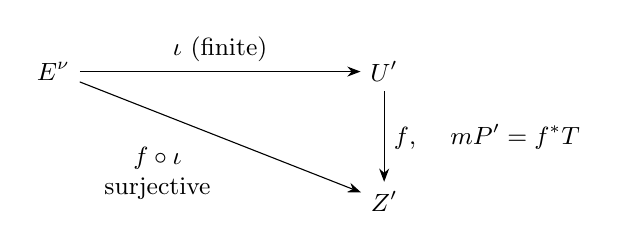
\begin{tikzpicture}[>=Stealth,baseline=(current bounding box.center),
 every node/.style={font=\small},x=1cm,y=1cm]
\node (E) at (0,1.65) {$E^\nu$};
\node (U) at (4.2,1.65) {$U'$};
\node (Z) at (4.2,0) {$Z'$};
\draw[->] (E) -- node[above] {$\iota$ (finite)} (U);
\draw[->] (U) -- node[right] {$f$, \quad $mP'=f^*T$} (Z);
\draw[->] (E) -- node[below left,align=center] {$f\circ\iota$\\surjective} (Z);
\end{tikzpicture}
\caption{The vertical case. The map $\iota$ is normalization followed
by inclusion. Surjectivity gives
$m\iota^*P'=(f\circ\iota)^*T\ne0$.
A prime component $J$ of this pullback maps finitely onto a
codimension-two subvariety of $U'$.}
\label{fig:vertical}
\end{figure}

Take a prime component $J$ of $P'|_{E^\nu}$. By
\cref{lem:adjunction}, its coefficient in the different
$C_{E^\nu}$ is positive and hence at least $1/n$. View $E^\nu$
over its own field of constants $k_E$. By \cref{lem:constants},
this is a normal geometrically integral projective variety of
dimension $d-1$ over $k_E$, with
\[
 [k_E:k]=\cdeg{E}{k}=\cdeg{E_3}{k}\leq M_{<d}(1).
\]
Since $k_E/k$ is finite separable, changing the ground field from
$k$ to $k_E$ does not alter its canonical divisor. The adjunction
pair is therefore a log Calabi--Yau pair over $k_E$. Induction in
dimension $d-1$ at threshold $1/n$ gives
\[
 \cdeg{J}{k_E}\leq N(d-1,1/n).
\]
As $k_E\subset k(J)$, degrees in the tower of constant fields
multiply, and hence
\begin{equation}\label{eq:Jbound}
 \cdeg{J}{k}=[k_E:k]\cdeg{J}{k_E}
 \leq M_{<d}(1)N(d-1,1/n).
\end{equation}

Finally work over $\kb$. Choose a geometric component $J_0$ of
$J$ and let $W_0$ be its image on $U'_{\kb}$. The normalization
map is finite, so $W_0$ has dimension $d-2$ and is contained in
a geometric prime component of $P'$. The geometric components
of $P'$ form a single Galois orbit. Thus every one of them
contains an image of a conjugate of $J_0$: conjugate both the
chosen containment and $J_0$.

There are at most $\cdeg{J}{k}$ such images. For each image,
\cref{lem:incidence} bounds by $2/b$ the number of components
of $P'_{\kb}$ that contain it, since all these components have
coefficient at least $b$ in $C'_{\kb}$ and $U'_{\kb}$ is
$\Q$-Gorenstein klt. Counting the incidences, with repeated images
only increasing the upper bound, yields
\begin{equation}\label{eq:final-incidence}
 \cdeg{S}{k}=\cdeg{P'}{k}
 \leq\frac2b\cdeg{J}{k}
 \leq\frac2b M_{<d}(1)N(d-1,1/n).
\end{equation}

\subsection{Uniformity and conclusion}

The four cases \eqref{eq:first-horizontal},
\eqref{eq:bounded-fano-case}, \eqref{eq:second-horizontal}, and
\eqref{eq:final-incidence} exhaust the proof. In particular, after
choosing $b=b(t)$ and $n=n(d,b)$, it suffices to take an integer
majorant of
\begin{equation}\label{eq:recurrence}
 \max\left\{
 \begin{aligned}
 &M_{<d}(t),\quad M_{<d}(b),\quad A(d,1/n,n),\\
 &\frac2b M_{<d}(1)N(d-1,1/n)
 \end{aligned}\right\}.
\end{equation}
Every inductive term involves a strictly smaller ambient dimension.
All thresholds and the complement index depend only on $d,t$.
Neither the field, any original coefficient denominator, the number
of extracted divisors, nor the auxiliary small perturbations enters
this maximum. Thus it defines a finite bound depending only on
$d,t$ and closes the induction.

For the original possibly nonnormal component $S$, the injection
$H^0(S,\OO_S)\hookrightarrow H^0(S^\nu,\OO_{S^\nu})$ now gives the
claimed Stein-degree bound. This proves \cref{thm:main}.\hfill$\square$

\begin{thebibliography}{BCHM10}
\bibitem[BMT11]{BMT2011}
E.~Bierstone, P.~D.~Milman, and M.~Temkin,
$\Q$-universal desingularization,
\emph{Asian J. Math.} \textbf{15} (2011), 229--250.
\href{https://doi.org/10.4310/AJM.2011.v15.n2.a5}{doi:10.4310/AJM.2011.v15.n2.a5}.

\bibitem[Bir19]{Birkar2019}
C.~Birkar, Anti-pluricanonical systems on Fano varieties,
\emph{Ann. of Math.} \textbf{190} (2019), 345--463.
\href{https://doi.org/10.4007/annals.2019.190.2.1}{doi:10.4007/annals.2019.190.2.1}.

\bibitem[Bir21]{Birkar2021}
C.~Birkar, Singularities of linear systems and boundedness of Fano varieties,
\emph{Ann. of Math.} \textbf{193} (2021), 347--405.
\href{https://doi.org/10.4007/annals.2021.193.2.1}{doi:10.4007/annals.2021.193.2.1}.

\bibitem[Bir26]{Birkar2026}
C.~Birkar, \emph{Stein degree of proper morphisms},
\href{https://arxiv.org/abs/2603.23939v1}{arXiv:2603.23939v1} (2026).

\bibitem[BCHM10]{BCHM2010}
C.~Birkar, P.~Cascini, C.~D.~Hacon, and J.~McKernan,
Existence of minimal models for varieties of log general type,
\emph{J. Amer. Math. Soc.} \textbf{23} (2010), 405--468.
\href{https://doi.org/10.1090/S0894-0347-09-00649-3}{doi:10.1090/S0894-0347-09-00649-3}.

\bibitem[BQ25]{BirkarQu2025}
C.~Birkar and S.~Qu, \emph{Stein degree on log Calabi--Yau fibrations},
\href{https://arxiv.org/abs/2509.20948v1}{arXiv:2509.20948v1} (2025).

\bibitem[Kol10]{KollarDraft}
J.~Koll\'ar, \emph{Canonical models}, author-hosted draft chapter,
June 1, 2010, Definition 122 and formulas (122.7)--(122.10), pp.~61--62.
\href{https://web.math.princeton.edu/~kollar/book/chap2.pdf}{Author's draft};
numbering is that of this draft, not the published book.

\bibitem[Kol13]{Kollar2013}
J.~Koll\'ar, \emph{Singularities of the Minimal Model Program},
with the collaboration of S.~Kov\'acs, Cambridge Tracts in Mathematics 200,
Cambridge University Press, 2013.
\href{https://doi.org/10.1017/CBO9781139547895}{doi:10.1017/CBO9781139547895}.

\bibitem[KM98]{KM1998}
J.~Koll\'ar and S.~Mori, \emph{Birational Geometry of Algebraic Varieties},
Cambridge Tracts in Mathematics 134, Cambridge University Press, 1998.
\href{https://doi.org/10.1017/CBO9780511662560}{doi:10.1017/CBO9780511662560}.

\bibitem[LM26]{LyuMurayama}
S.~Lyu and T.~Murayama, \emph{The relative minimal model program for
excellent algebraic spaces and analytic spaces in equal characteristic zero},
\href{https://arxiv.org/abs/2209.08732v4}{arXiv:2209.08732v4} (2026),
forthcoming in \emph{Memoirs of the European Mathematical Society}.
\end{thebibliography}
\end{document}
